\documentclass[11pt]{report}
\usepackage{fullpage}
%\usepackage{sourcesanspro, sourcecodepro}
\usepackage{minted}
\usepackage{graphicx}
\usepackage{awesomebox}
\usepackage{hyperref}
\usepackage{float} % stops images from moving around
\usepackage[a4paper, total={6in, 8in}, margin=0.75in]{geometry}
\usepackage{etoolbox}
\makeatletter
\patchcmd{\chapter}{\if@openright\cleardoublepage\else\clearpage\fi}{}{}{}
\RequirePackage[T1]{fontenc}
\RequirePackage[default,light,black]{roboto}

\hypersetup{
    colorlinks=true,
    linkcolor=blue,
    citecolor=blue,
    filecolor=blue,
    urlcolor=blue,
    pdfborder={0 0 0}
}

\graphicspath{{./images/}}

\title{APSC 258: Lab 4 Manual}
\author{Andre Cox \\ Scott Halston}

\begin{document}
\maketitle
\tableofcontents

\clearpage

\chapter{Introduction}
Over the next four lab sections, you will be tasked with creating your own neural networks. To do this, each of the next four labs will be building upon each other by teaching you how to apply every component of a neural network one-by-one. Your ultimate goal will be to create the most accurate, fast, and efficient neural networks; but, for now, your goal for each lab should be to mess around with parameters to build your understanding of how each component affects each other.

\section{Introduction}
In this lab, we will be creating a simple neural network to predict the steering angle of the car.
By the end of this lab, you should have a network that can drive the car and follow the lane lines. Some parts of making neural networks are out of the scope of this course, so we will provide you with a starting point for your work. You do not need to, though, if you are curious, you can download the code for this lab from the
\href{https://github.com/PiCarV/Demos}{Github Repository}.

\section{Understanding Dense Layers}
Dense layers are the most basic type of neural network layer. They are simply a layer of neurons that are connected to each other. The neurons in a dense layer are simply a weighted sum of the inputs. The weights are adjusted until the network is able to predict the correct output. The process of updating the weights is called backpropagation. Generally, the more neurons and layers you have, the more accurate the network will be. 

\section{Google Colab} 
We can train our neural networks using our computers; however, this will probably be slow depending on your computer's power. To solve this hardware bottleneck, we will use a service called \href{https://colab.research.google.com/}{Google Colab}. This service provides a cloud-based platform for training neural networks and it is free for basic use. You will need a Google account in order to be able to train your own neural networks. This Lab document will walk you through how to use Google Colab but first, we must talk about theory.

\pagebreak

\section{Data}
We will be using 2 datasets. The first is a training dataset that we will use to train our neural network. The second is a test dataset that we will use to test our neural network (validation data). You can download the datasets from Canvas labled as "TrainingData.7zip" and "TestingData.7zip". 

\warningbox{
    \textbf{Caution: }
    These files are compressed using 7zip. Do not extract this compressed file because our provided code will extract the files for you. We will show you how to do this in the next section.
}
\chapter{Dense Layers Deep Dive}
\section{How dense layers work in practice}
Dense layers are an array of weights that are placed side by side. Multiple layers of dense layers can be connected together by connecting each weight in the previous layer to the weight in the next layer. This may look something like this:

% insert figure

    \begin{figure}[h]
        \begin{center}
        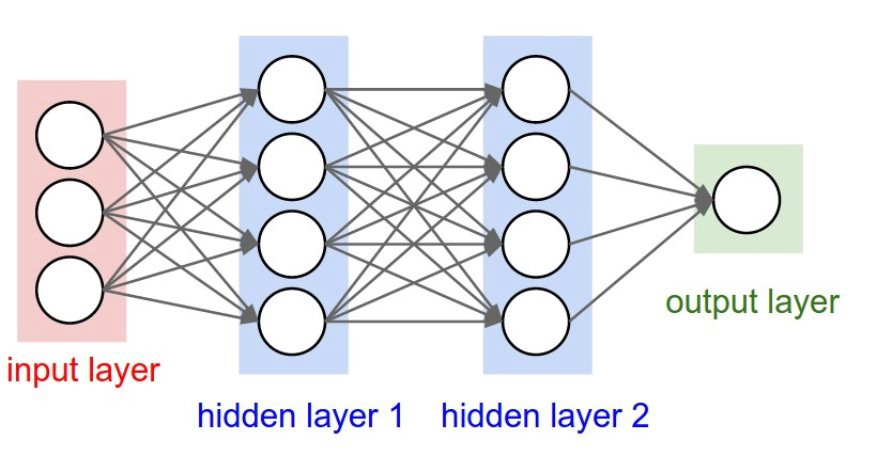
\includegraphics[width=0.4\textwidth]{denselayers.jpeg}
        \caption{Dense layers visualization}
        \label{fig:dense_layers}
        \end{center}
    \end{figure}

The weights in each neuron in the dense layer are activated by the inputs. The activation of the neuron is the weighted sum of the inputs. The activation of the neuron is then passed through a non-linear activation function to get the output. The output of the neuron is then connected to the next layer. There are many different activation functions that can be used. A couple of common ones are displayed below.
\begin{center}
    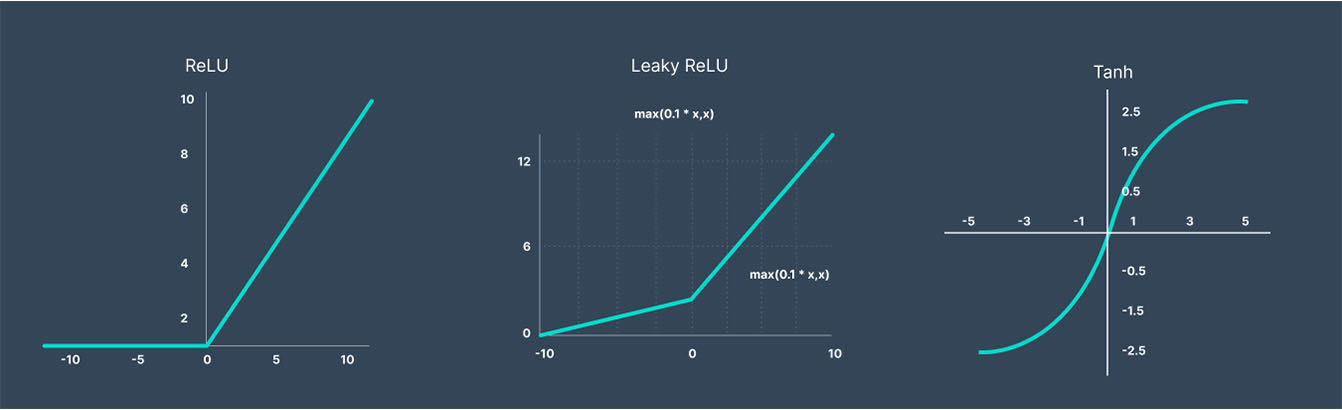
\includegraphics[width=0.7\textwidth]{activation functions 1.jpg}
\end{center}

\begin{figure}
    \begin{center}
    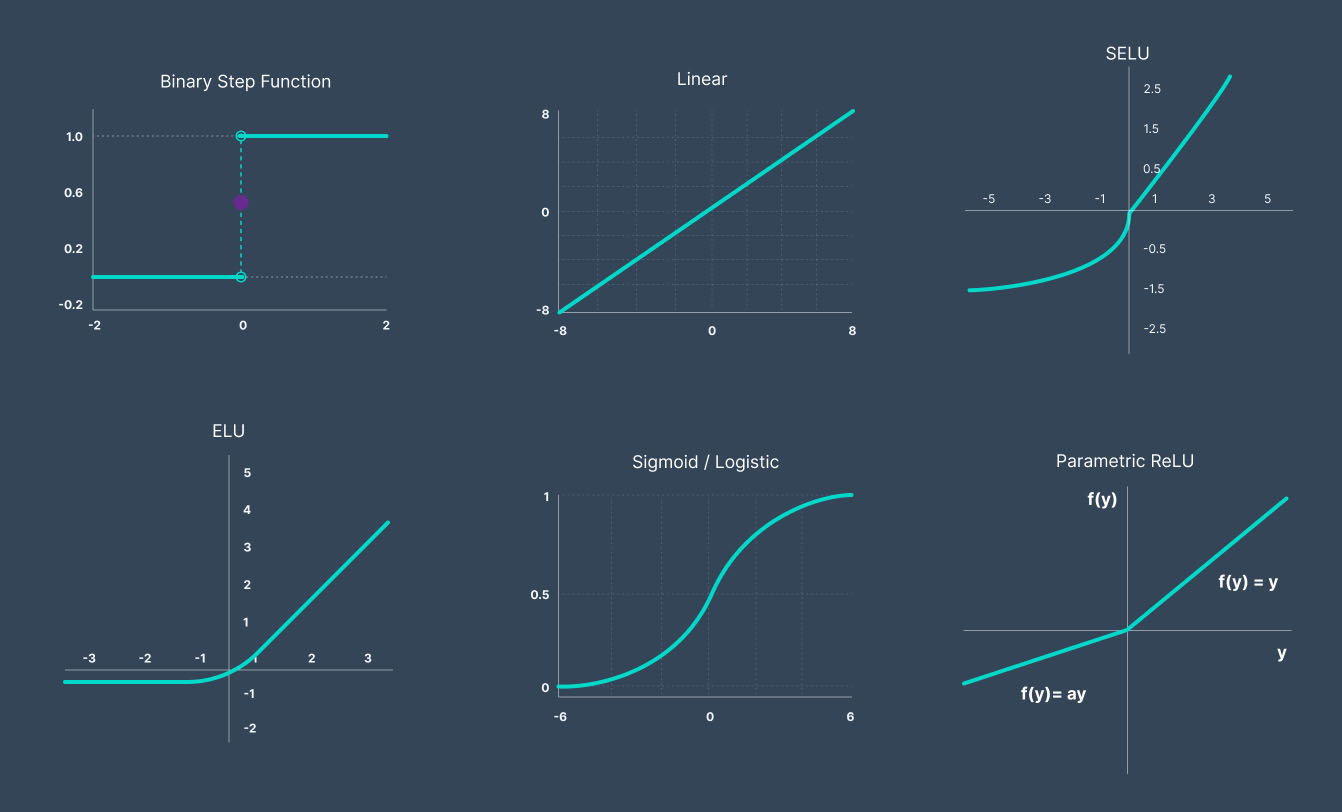
\includegraphics[width=0.7\textwidth]{activation functions 2.jpg}
    \caption{Common activation functions}
    \label{fig:activation_functions}
    \end{center}
\end{figure}

\section{Using Dense Layers in Keras}
Keras is the Python library that we will use to create our neural networks. Keras is a high level library that allows us to create neural networks in a simple and easy way. Later you will see that we provide a pre-made template for you to use. However, you still need to understand how to create a neural network in Keras.

\pagebreak

\chapter{Start of the Lab}
Before we can begin to mess with dense layers, we will learn how to get started with Google Colab. To begin, go to the \href{https://accounts.google.com/v3/signin/identifier?dsh=S1644191332%3A1675546780545376&continue=https%3A%2F%2Fcolab.research.google.com%2F&ec=GAZAqQM&passive=true&flowName=GlifWebSignIn&flowEntry=ServiceLogin&ifkv=AWnogHeZG2rpE0K9cdZU_E4kGDMUnn6If0bNDxEje1kgybK3_oj12LJ91m-WjXqGeI5Ljbego94BOQ}{Google Colab} website and either sign in with an existing Google account or sign up for an account.

\begin{center}
    
\includegraphics[scale=0.5]{signinup.png}
\end{center}

Once you are signed in, there is an important setting we must change before continuting. Click on the drop down tab named "Runtime" at the top of the Google Colab page and then select "Change runtime type". A window will open and we want to change the "Hardware accelerator" option from "None" to "GPU". Once "GPU" is selected, make sure you click "Save".

\begin{center}
    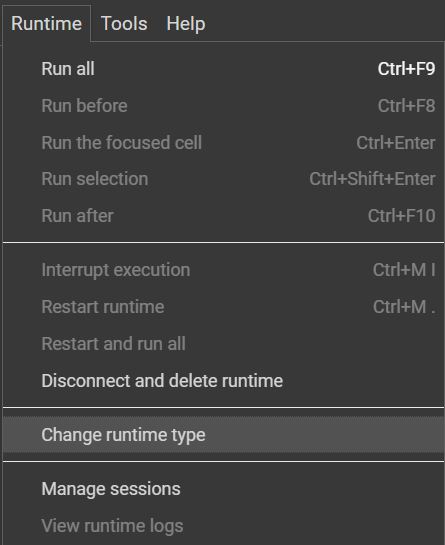
\includegraphics[scale=0.3]{runtime.png}
    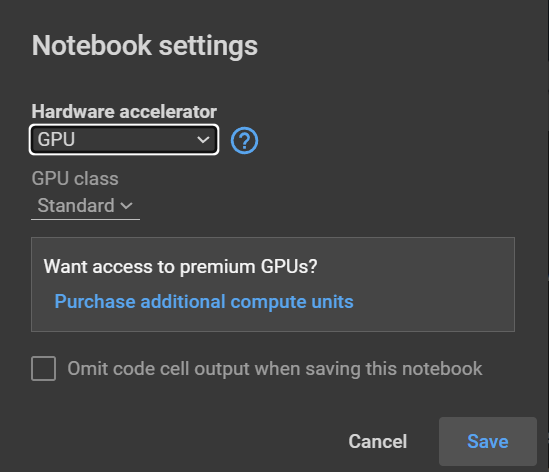
\includegraphics[scale=0.4]{runtimegpu.png}
\end{center}

Our next step is to open the provided demo model in Google Colab. To do this, click on the drop down tab named "File" at the top of the Google Colab page and then select "Upload notebook" as shown below.

\begin{center}
    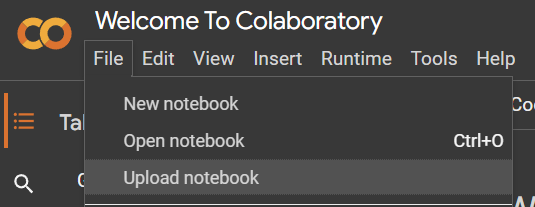
\includegraphics[scale=0.6]{creataproject.png}
\end{center}

This will open a page with a few differnt options. Select the tab called "GitHub" at the top of the window. Next, Paste the following link as shown in the image below.\newline

\url{https://github.com/PiCarV/Demos/blob/main/Lab%20Code/Lab%20Part%204/model.ipynb} \newline

Lastly, click "Lab Code/Lab Part 4/model.ipynb" and the demo model will open.

\begin{center}
    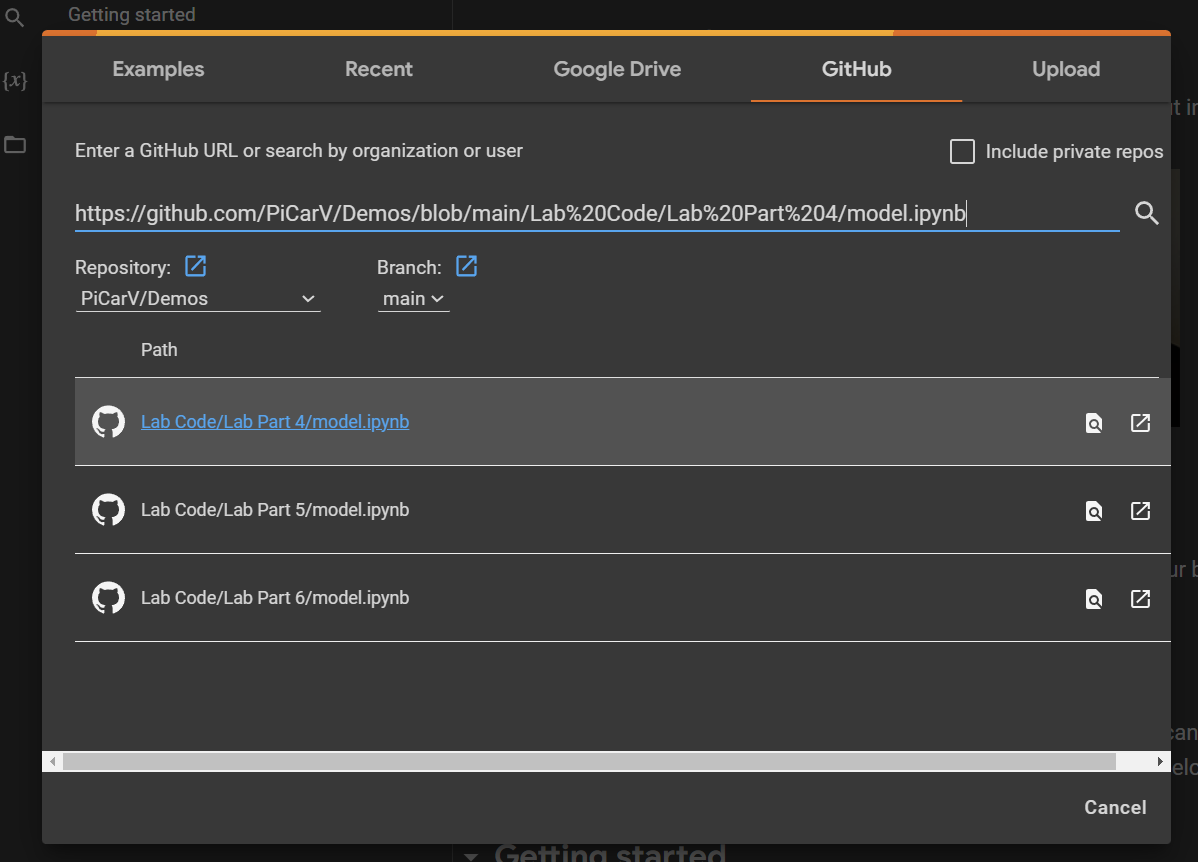
\includegraphics[scale=0.3]{openmodel.png}
\end{center}

\section{Data Upload}
Now we will upload the training and test datasets to Google Colab. To do this, take the file you download from Canvas named "TrainingData.7zip" and upload it to your \href{https://drive.google.com/drive}{Google Drive}.
Please make sure that you are signed into the same Google account as your Google Colab and that you do not put the training data into any folders. The TrainingData.7zip file should be at the surface of your Google Drive as shown below.

\begin{center}
    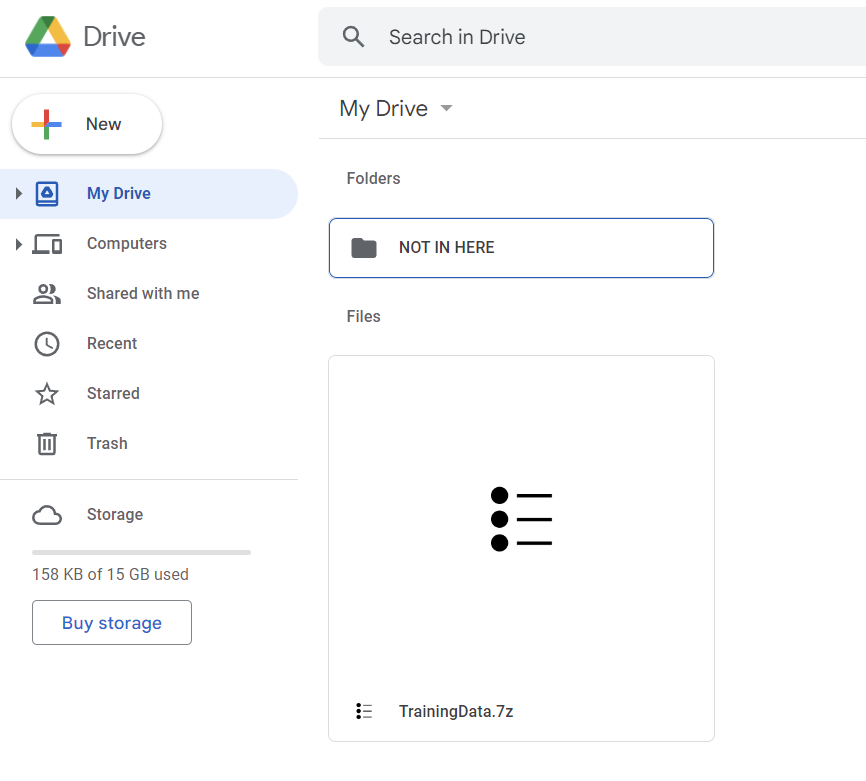
\includegraphics[scale=0.5]{trainingdata.png}
\end{center}

\chapter{Running the Code}
Now that Google Colab is set up and your data is uploaded, you can run the code. Simply open the model.ipynb file, click "Connect" at the top right of the page, and then run each code block one by one; make sure to wait for the previous code blocks to finish before running the next.

\begin{center}
    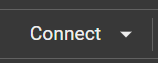
\includegraphics[scale=0.4]{connect.png}
\end{center}

\section{Building your network}
Once you get to Part 4 of the code, you are ready to build your neural network. You can modify the code provided to try to get a better training result. Your goal should be to have a small mean squared error (MSE) value and consistent validation accuracy. To do this you can try adding more layers, changing the activation functions, or changing the number of neurons in the hidden layers.

\section{Saving the network}
After you have trained your neural network, you can save it to a file. To do this, simply run the final code block. Before you do this, we recommend changing the name of the file to something more meaningful. After this block runs you can find a file called model.h5 or whatever you decided to name on the left files tab in Google Colab. Refer to the image below. This is the file that the Pi Car V will use to self-drive. You should right-click on the model.h5 file and download it to your computer. 

\begin{center}
    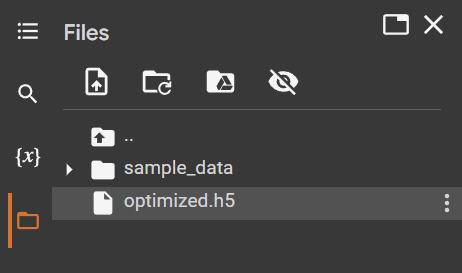
\includegraphics[scale=0.6]{savved.png}
    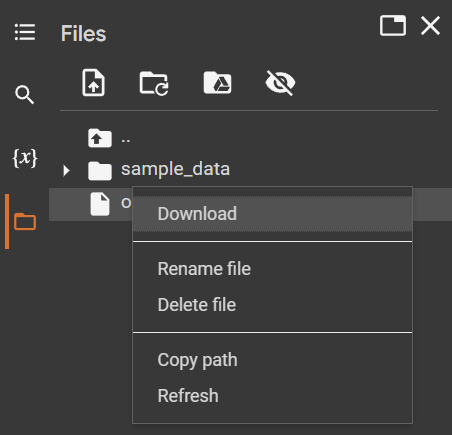
\includegraphics[scale=0.6]{downloadh5.png}
\end{center}


\chapter{Running the Pi Car V} 
Now that you have trained your neural network, you can run the Pi Car V. You should already have all the required dependencies installed. If you haven't, you can go back to lab 2.
Next, we can download the software for running your network on the Pi Car V. This software is provided for you as writing this code yourself could be a bit of a challenge. You can find the script
\href{https://raw.githubusercontent.com/PiCarV/CarRunner/main/carRunner.py}{carRunner.py} here. This will open in your default web browser. You can then right click and select "Save As...". Save the file somewhere on your computer.
You can open the file in VSCode, then you can click on Terminal -> New Terminal. This will open a new terminal window. Now you just need to add your model.h5 file to the same directory and run the script.
\begin{minted}[]{bash}
python runNetwork.py
\end{minted}
If your file is named something else, you can add some command line arguments to the file. For example
\begin{minted}[]{bash}
python runNetwork.py --model differentModel.h5    
\end{minted}
For a full list of command line arguments, you can type: 
\begin{minted}[]{bash}
python runNetwork.py --help
\end{minted}
\section{Control the Pi Car V}
Once the “runNetwork” file is running, a window will open. You can use this window to adjust the speed of the car and the color mask.

\section{Finishing Up}
To complete this lab, you will need to experiment to get your car to follow the lane lines. This will be a bit tricky and it is okay if it is not perfect. Next lab we will introduce a new layer type that will help you achieve a better neural network.

\end{document}